\chapter{Calcul d'un ombrage expressif pour les panoramas}

\section{Vue d'ensemble de la solution}

Notre objectif est de faire un rendu 3D temps réel des ombres d'un panorama dans le style de l'atelier Novat. Comme vu dans l'étude du style de Pierre Novat, les ombres jouent un grand rôle dans lecture du panorama et mettent en valeur la forme de la montagne. Pour correspondre à ce style, notre rendu des ombres doit donner à voir le maximum de variation dans le terrain et ainsi améliorer la perception des formes de la montagne par l'utilisateur. En d'autres termes, lorsque le terrain est lisse, il faut voir que c'est plat et lorsqu'il y a des variations dans le terrain, petites ou grandes, il faut pouvoir les voir sans pour autant en rajouter artificiellement. Ces variations nous les appellerons aspérités.


Pour pouvoir construire notre modèle d'ombrage, nous nous appuyons sur un ensemble de règles qui résultent de nos études sur la cartographie et les œuvres de l'atelier Novat :

\begin{enumerate}
\item La lisibilité est privilégiée par rapport à la cohérence. 
\item La lumière a une direction générale qui vient d'en haut, à droite ou à gauche, de l'image. 
\item La direction peut être ajustée localement pour avoir une meilleure illumination de la zone.
\item Quand les ombres sont générées en utilisant un ordinateur, Tom Patterson conseille de faire deux ombrages différents puis de les fusionner pour garder le meilleur des deux. 
\item Les ombres portées sont moins présentes que l'ombrage.
\item Il n'y a pas de réflexion spéculaire.
\end{enumerate}

L'intuition derrière notre solution est la suivante : une fois une direction générale de la lumière choisie par l'utilisateur, nous la corrigeons localement afin de donner à voir au mieux les aspérités. Pour cela nous proposons de faire en sorte que chaque aspérité ait une face éclairée et une face à l'ombre tout en conservant l'orientation générale de la lumière, c'est-à-dire que la face en lumière doit rester du coté de la lumière principale. Pour appliquer cette correction, nous nous occupons uniquement d'ajuster l'azimut (c'est à dire l'orientation de la lumière par rapport au Nord). et nous ne touchons pas à l'élévation. Nous obtenons ainsi un ombrage localement ajusté et globalement cohérent. 
Cependant, comme les aspérités se répartissent sur plusieurs échelles : les petites aspérités se confondent avec les plus grandes et se mélangent, nous suivons la règle (4.) et proposons d'utiliser deux échelles sur lesquelles nous calculons deux ombrages que nous fusionnons pour obtenir l'ombrage final. Enfin nous ajoutons une couche d'ombres portées plus discrète qui souligne le relief global.

En pratique nous prenons en entrée une carte de hauteur (modèle numérique de terrain) et nous travaillons en espace image, le terrain vu de dessus étant dans le plan $xy$.



\section{L'orientation de la lumière}



Notre modèle d'illumination est le modèle Lambertien. Le calcul de l'ombrage s'obtient par le produit scalaire entre un vecteur de lumière $\vec{l}$ et la normale $\vec{n}$ de la surface courante :
\begin{equation} 
D = \vec{l}\cdot{\vec{n}}\end{equation}

Pour améliorer la perception de la forme, nous modifions localement la direction de la lumière pour s’assurer de voir toutes les aspérités. En plaçant la lumière perpendiculairement à la pente , nous nous assurons de toujours produire une zone ombrée et une zone éclairée (Fig. \ref{fig:correction}). 
\begin{figure}[!h]
\centering 
        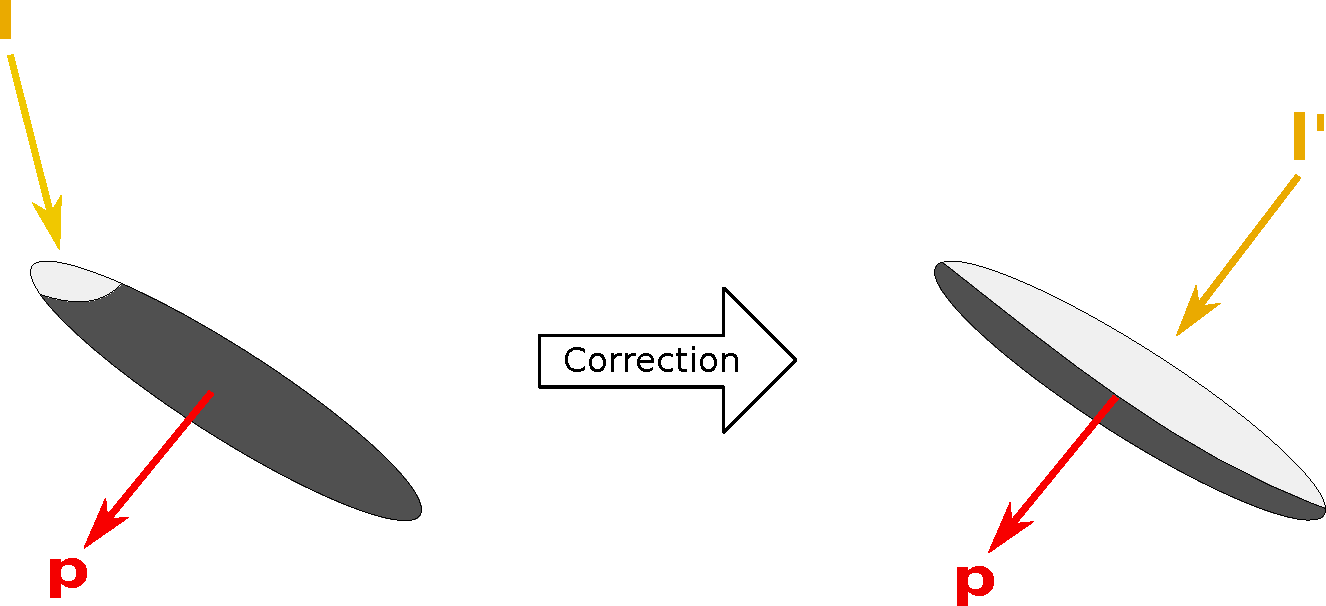
\includegraphics[width=0.4\linewidth]{Solution/correction_light.pdf}
        \caption{\label{fig:correction} Correction local sur un galet de la lumière $\vec{l}$ à l'aide de la pente $\vec{p}$ }
\end{figure}
%\jhon{C'est l'}
Notre problématique est donc de corriger l'azimut de $\vec{l}$ qui est sa projection sur le plan $xy$ que nous appellerons $\vec{l}_a$. En définissant le vecteur lumière par ses coordonnées polaires, les deux angles d'Euler : $\alpha$ et $\gamma$ (Fig. \ref{fig:euler}), la question revient à appliquer une correction $\theta$ à l'angle $\alpha$ locale en fonction d'une direction principale, tout en conservant $\gamma$. Cette direction principale est la pente $\vec{p}$ qui est définie par le gradient de la carte de hauteur, en d'autre terme, la normale projetée sur le plan $xy$. Donc nous calculons l'angle $\theta$ entre l'azimut du vecteur lumière $\vec{l}_a$ et la pente $\vec{p}$, pour l'appliquer ensuite à $\alpha$ et recalculer un vecteur lumière local $\vec{l'}$


\begin{figure}[!h]
\centering 
        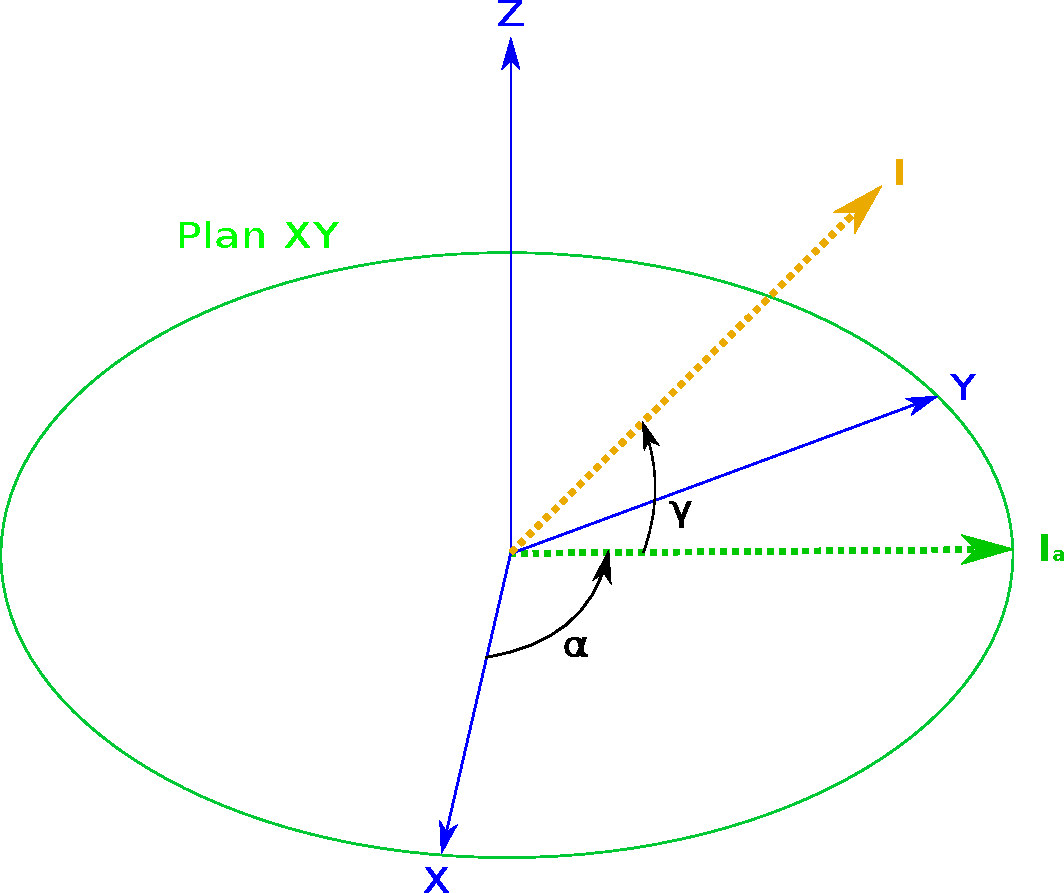
\includegraphics[width=0.3\linewidth]{Solution/euler_V3.pdf}
        \caption{\label{fig:euler} Angles d'Euler du vecteur lumière $\vec{l}$ avec $\vec{l}_a$ sa projection sur le plan $xy$ }
\end{figure}

Dans un 1er temps, nous cherchons à aligner parfaitement la lumière $\vec{l}$ avec la pente $\vec{p}$ , mais nous voulons aussi garder une cohérence globale c'est à dire que nous ne voulons pas que la direction de $\vec{l}$ se renverse totalement . Pour cela nous calculons  $\widehat{\vec{l}_a,\vec{q}}$ avec $\vec{q}$ la pente signée dans le sens de la lumière. Ainsi nous nous assurons que $\widehat{\vec{l}_a,\vec{q}}$ soit $\leq \pi $ :
\begin{equation}
\label{equationReverseN}
\vec{q} = 
	\left\{
    \begin{array}{ll}
        -\vec{p} & \mbox{si } \widehat{\vec{l}_a,\vec{p}} \leq \pi\\
		\vec{p} & \mbox{sinon}				
    \end{array}
\right.
\end{equation}


Ensuite nous calculons l'angle $\theta$ entre $\vec{l}_a$ et $\vec{q}$ en signant avec le déterminant $\Delta$ pour que $\theta$ soit dans l'intervalle  $-\frac{\pi}{2}$ et $\frac{\pi}{2}$ :
\begin{equation}
\label{equationAngleOri}
 \theta = \frac{\Delta}{|\Delta|} \arccos( \vec{l}_a \cdot{\vec{q}}) \ 
 \mathrm{avec} \  
\Delta =  \vec{l_{a_x}}\vec{q_y} - \vec{l_{a_y}}\vec{q_x}
\end{equation}

Enfin nous pouvons reconstruire le vecteur lumière ajusté localement grâce à une matrice de rotation :
\begin{equation}
\label{equationRotationMat}
\vec{l'} = 
\begin{pmatrix}
x \\
y \\
z \\
\end{pmatrix}
=
\begin{pmatrix}
\cos \gamma  \cos \alpha + \theta\\
\sin \gamma \\
\cos \gamma  \sin \alpha + \theta \\
\end{pmatrix}
\end{equation}



\begin{figure*}[h!]
\centering
 \begin{subfigure}[t]{0.47\textwidth}
 \centering
 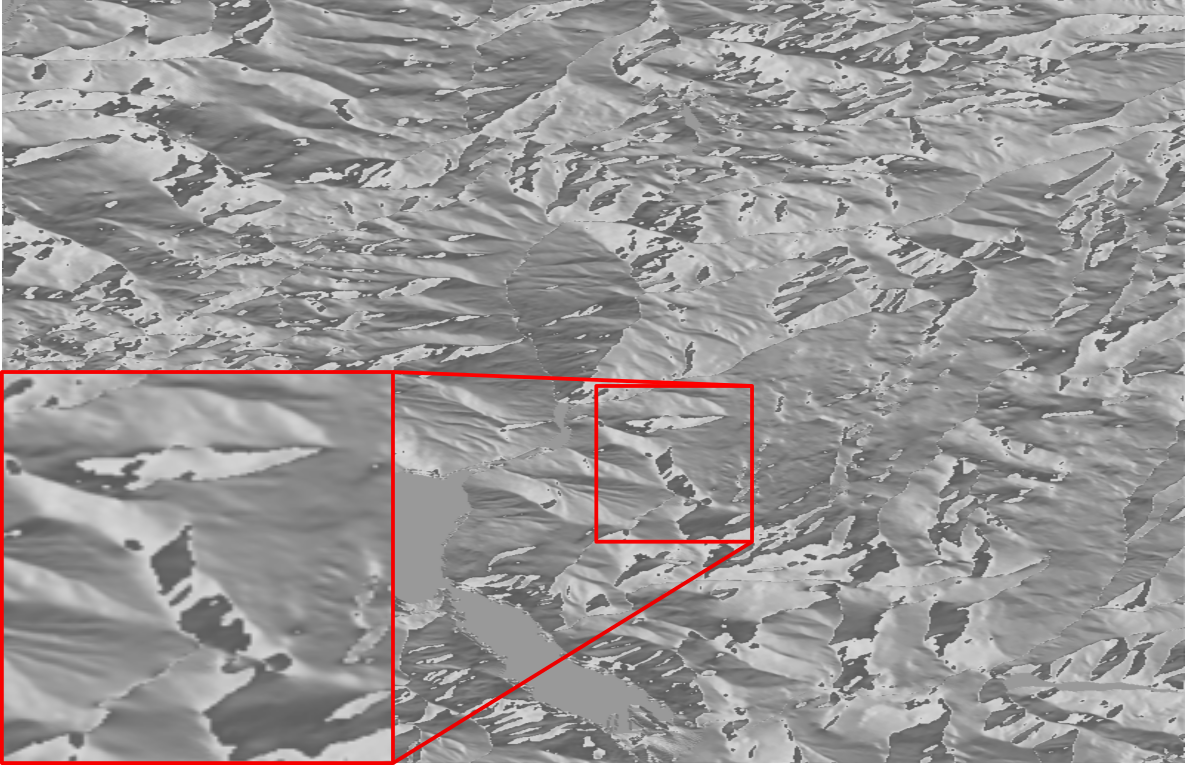
\includegraphics[width=1.0\linewidth]{Solution/theta_discontinu.png}
 \caption{$\theta$ en niveau de gris}
 \end{subfigure}
 \begin{subfigure}[t]{0.47\textwidth}
 \centering
 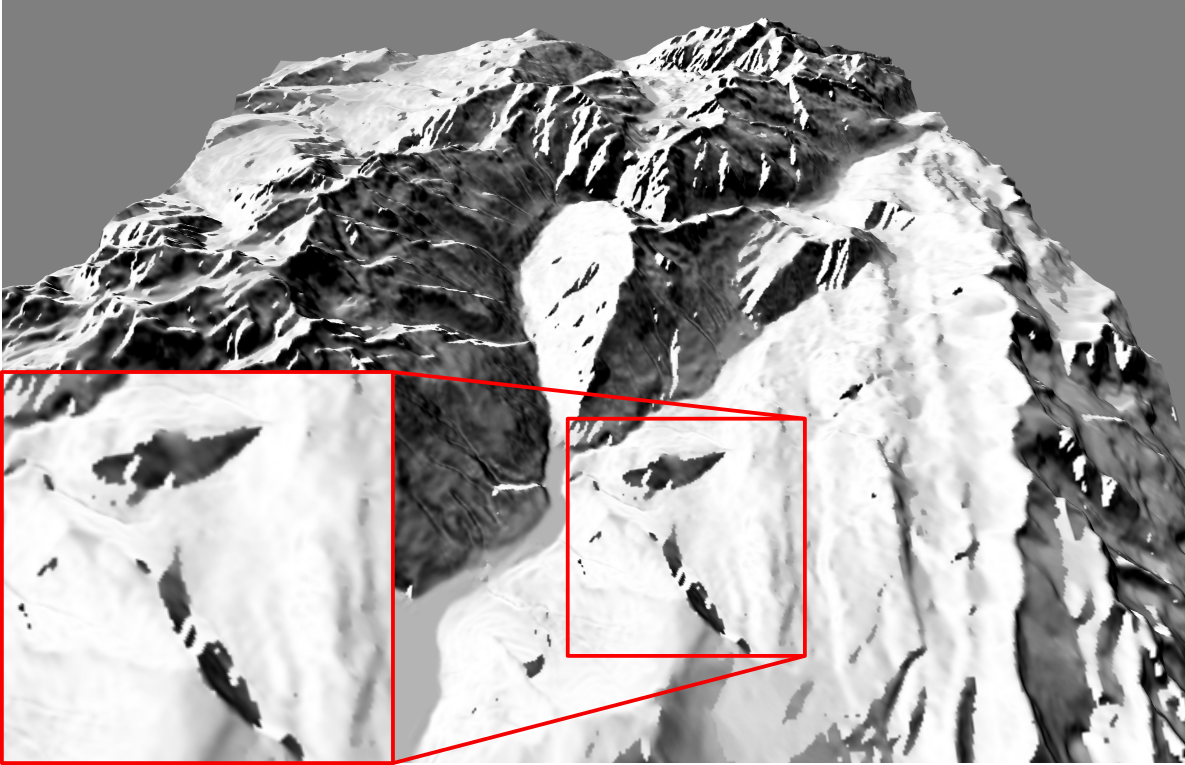
\includegraphics[width=1.0\linewidth]{Solution/ombrage_discontinue.png}
 \caption{Ombrage avec correction de la lumière}
 \end{subfigure}
 \caption{\label{fig:shadingDiscontinu}Exemple de correction de la lumière sur un terrain ($\alpha = 45\degres$ (Nord-Ouest), $\gamma = 45 \degres$) . Nous constatons que la lumière s’aligne bien avec les aspérité mais aux prix de discontinuité. }
\end{figure*}





À ce stade, comme nous pouvons le constater sur la Figure \ref{fig:shadingDiscontinu}, il y a des discontinuités dans le vecteur lumière qui ont deux causes differentes :
\begin{enumerate}
\item $\theta$ passe d'un seul coup de $-\frac{\pi}{2}$ à $\frac{\pi}{2}$ et inversement  
\item Quand $\vec{p'}$ est nul, il est possible que ses voisins soit très petits mais pas dans le même sens. 
\end{enumerate}

Pour corriger la première discontinuité nous multiplions $\theta$ avec une interpolation d’Hermite qui va permettre d'interpoler $\theta$ de manière continue  entre $-\frac{\pi}{2}$ et $\frac{\pi}{2}$. Cette interpolation se fait en deux étapes. 

Dans un premier temps nous calculons $S(x)$ qui va limiter la valeur de $|\theta|$ entre $T$ et $\frac{\pi}{2}$ et inverser cet intervalle. C'est-à-dire que lorsque de $|\theta|$ $\leq T$, alors l'interpolation nous renvoie :
\begin{equation}
\label{equationClamp}
S(x) = 
	\left\{
    \begin{array}{ll}
        0 & \mbox{si } x \leq 0 \\
		x & \mbox{si } 0 \leq x \leq 1 \\
        1 & \mbox{si } 1 \leq x \\
    \end{array}
\right.
\mathrm{avec} \  
x = - \frac{|\theta| - T}{\frac{\pi}{2}-T} + 1 
\end{equation}

Note : $T$ est une limite laissée au choix de l'utilisateur, elle peut être entre $0$ et $\frac{\pi}{2}$ où à $0$, il n'y a aucune correction de lumière qui est faite et à $\frac{\pi}{2}$ la correction est maximale. Cependant pour le reste du rapport $T = \frac{\pi}{3}$ qui est le meilleur choix pour avoir une bonne correction sans avoir de discontinuité importante.


Ensuite, nous calculons le polynôme d'Hermite pour avoir un facteur continu entre $0$ et $1$ : 
\begin{equation}
\label{equationHermite}
H(x) = 3S(x)^2 - 2S(x)^3 
\end{equation}

Pour corriger la seconde discontinuité, nous utilisons simplement la norme de la projection de $\vec{n}$ sur le plan $xy$, c'est à dire $||\vec{p}||$.  Cela permet d’éviter d'avoir des faibles corrections lorsque la normale est presque verticale.
Ainsi nous ajoutons une étape entre  \eqref{equationAngleOri} et \eqref{equationRotationMat} :
\begin{equation}
\theta' = \theta \ . \ H(|\theta|) \ . \ ||\vec{p} ||
\end{equation}





\begin{figure*}[h!]
\centering
 \begin{subfigure}[t]{0.47\textwidth}
 \centering
 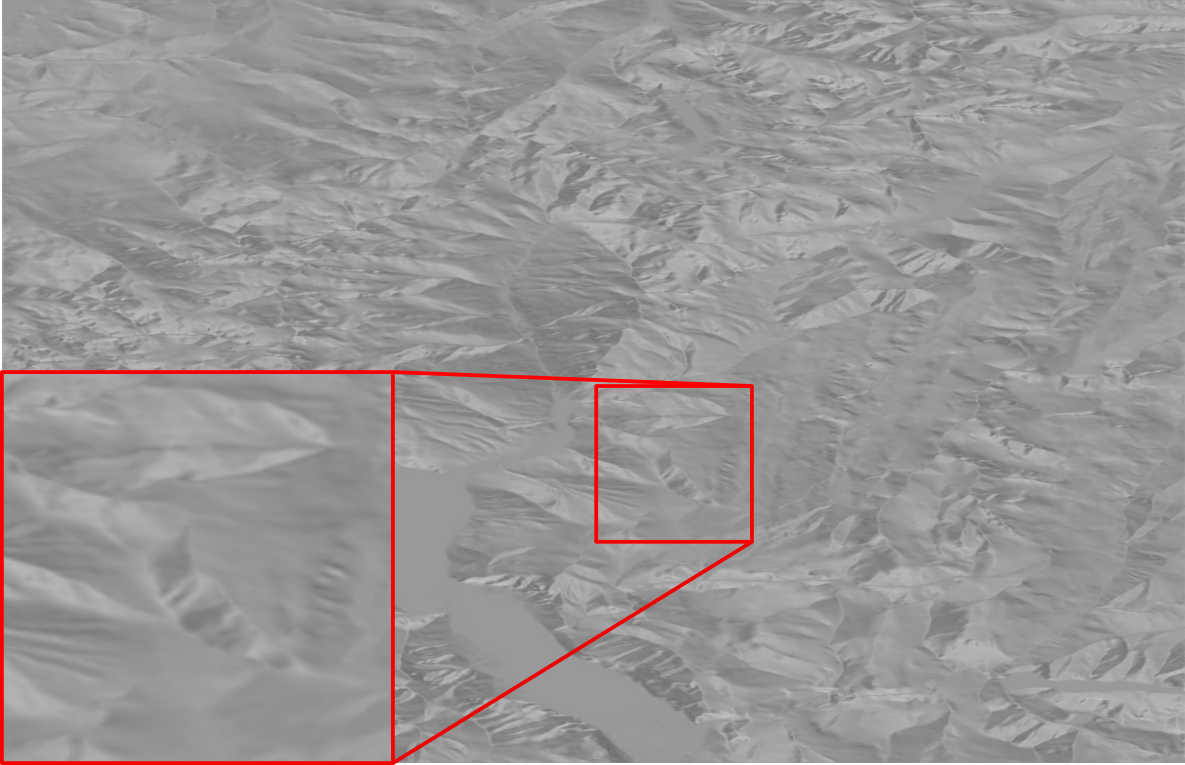
\includegraphics[width=1.0\linewidth]{Solution/theta_continu.png}
 \caption{$\theta$ en niveau de gris}
 \end{subfigure}
 \begin{subfigure}[t]{0.47\textwidth}
 \centering
 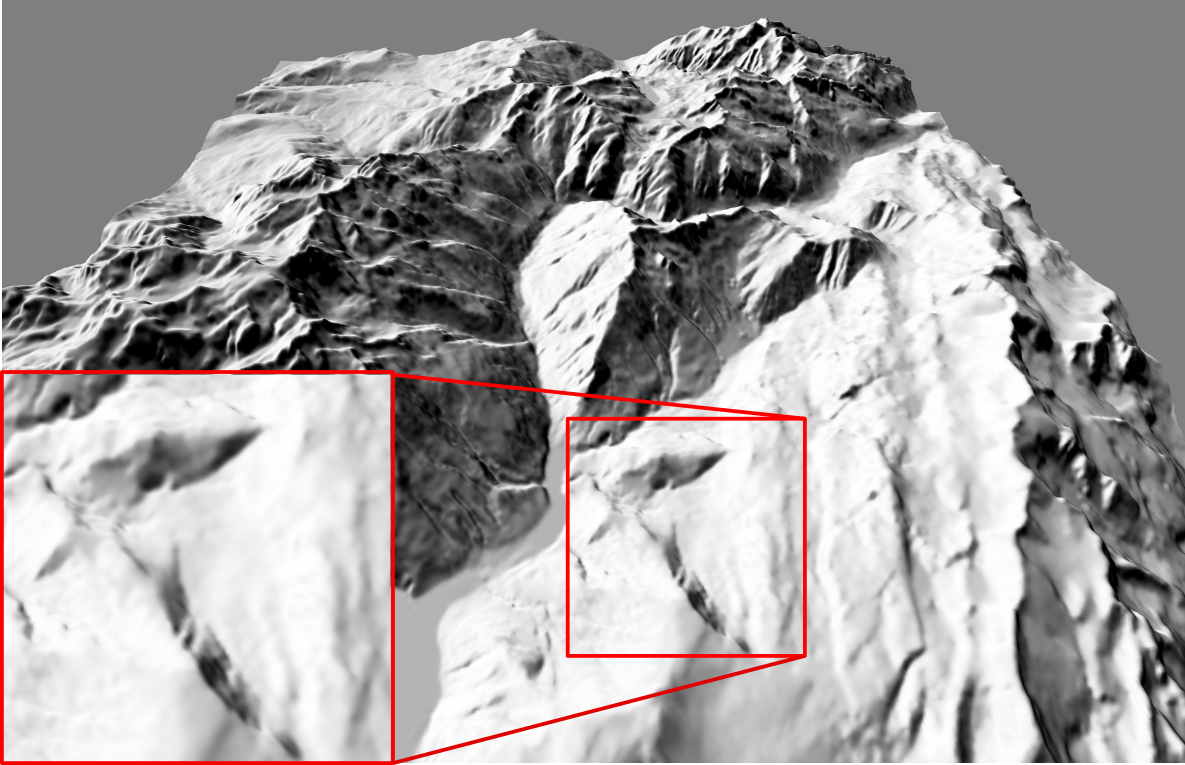
\includegraphics[width=1.0\linewidth]{Solution/ombrage_continue.png}
 \caption{Ombrage avec correction de la lumière}
 \end{subfigure}
 \caption{\label{fig:shadingContinu}Exemple de correction de la lumière sur un terrain sans les discontinuités ($\alpha =  45\degres$ (Nord-Ouest), $\gamma = 45\degres$). Le résultat est bien plus continue sans pour autant casser la correction.}
\end{figure*}


\section{L'ombrage multi échelle}

Une fois l'orientation locale de la lumière faite, il se pose un nouveau problème. En effet, nous alignons la lumière par rapport à la pente, or la direction de cette pente est majoritairement influencée par la forme de la montagne et non par les petites aspérités qui sont dessus. En d'autres termes, avec cette méthode nous obtenons des montagnes blanches d'un coté, sombres de l'autre sans pouvoir percevoir les petites aspérités. 
\begin{figure*}[h!]
 \begin{subfigure}[t]{0.47\textwidth}
 \centering
 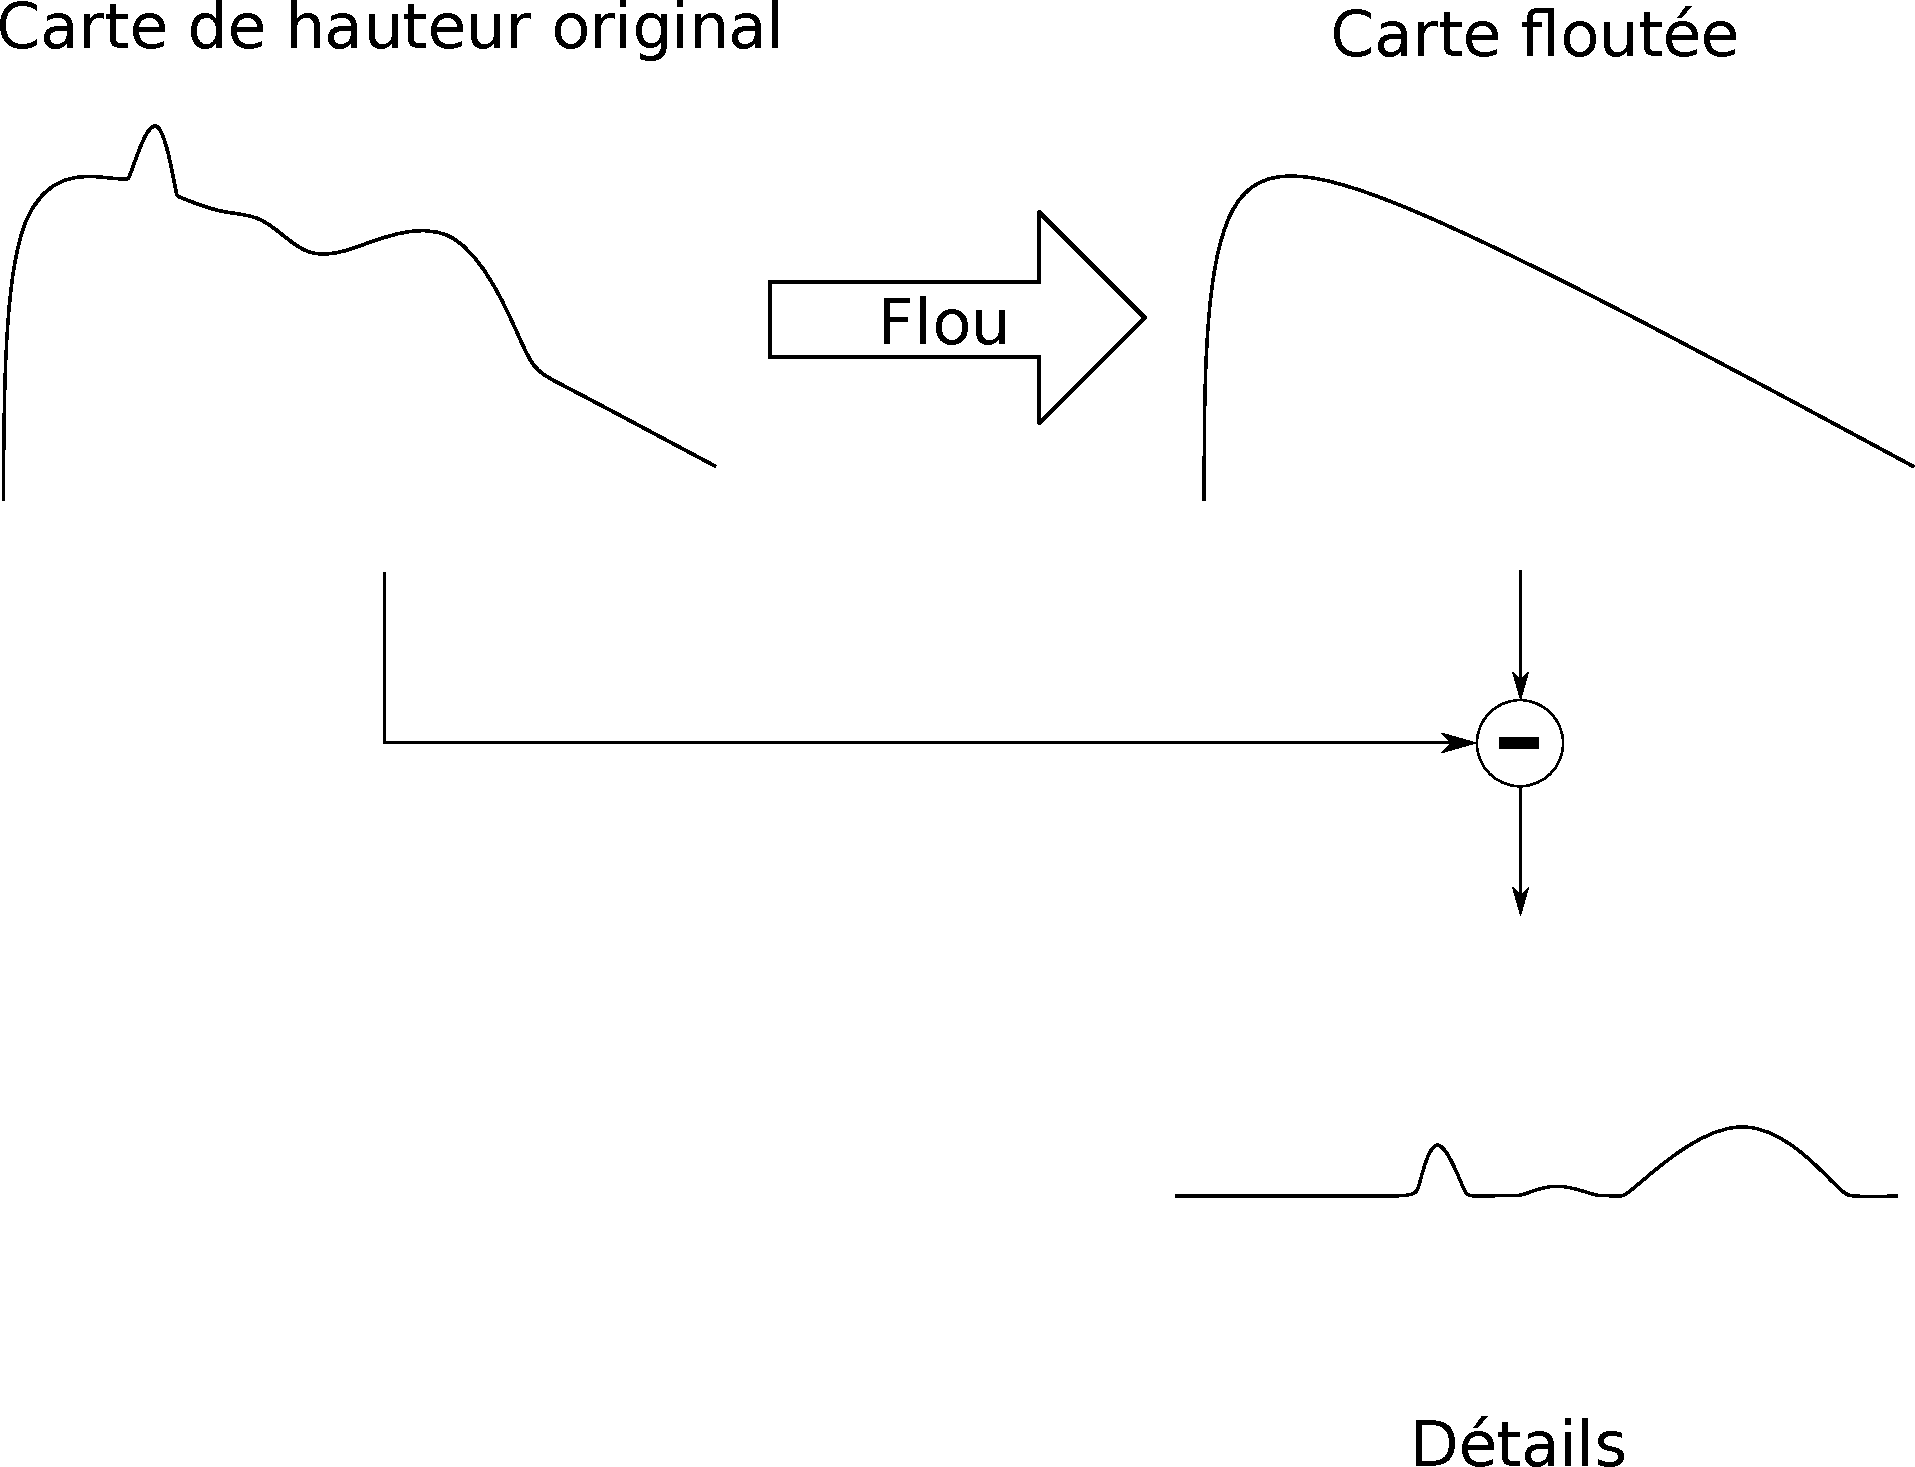
\includegraphics[width=1.0\linewidth]{Solution/pyramide_Laplace_schema.pdf}
 \caption{Une dimension}
 \end{subfigure}
   ~
 \hspace{.05\textwidth}
  \begin{subfigure}[t]{0.47\textwidth}
 \centering
 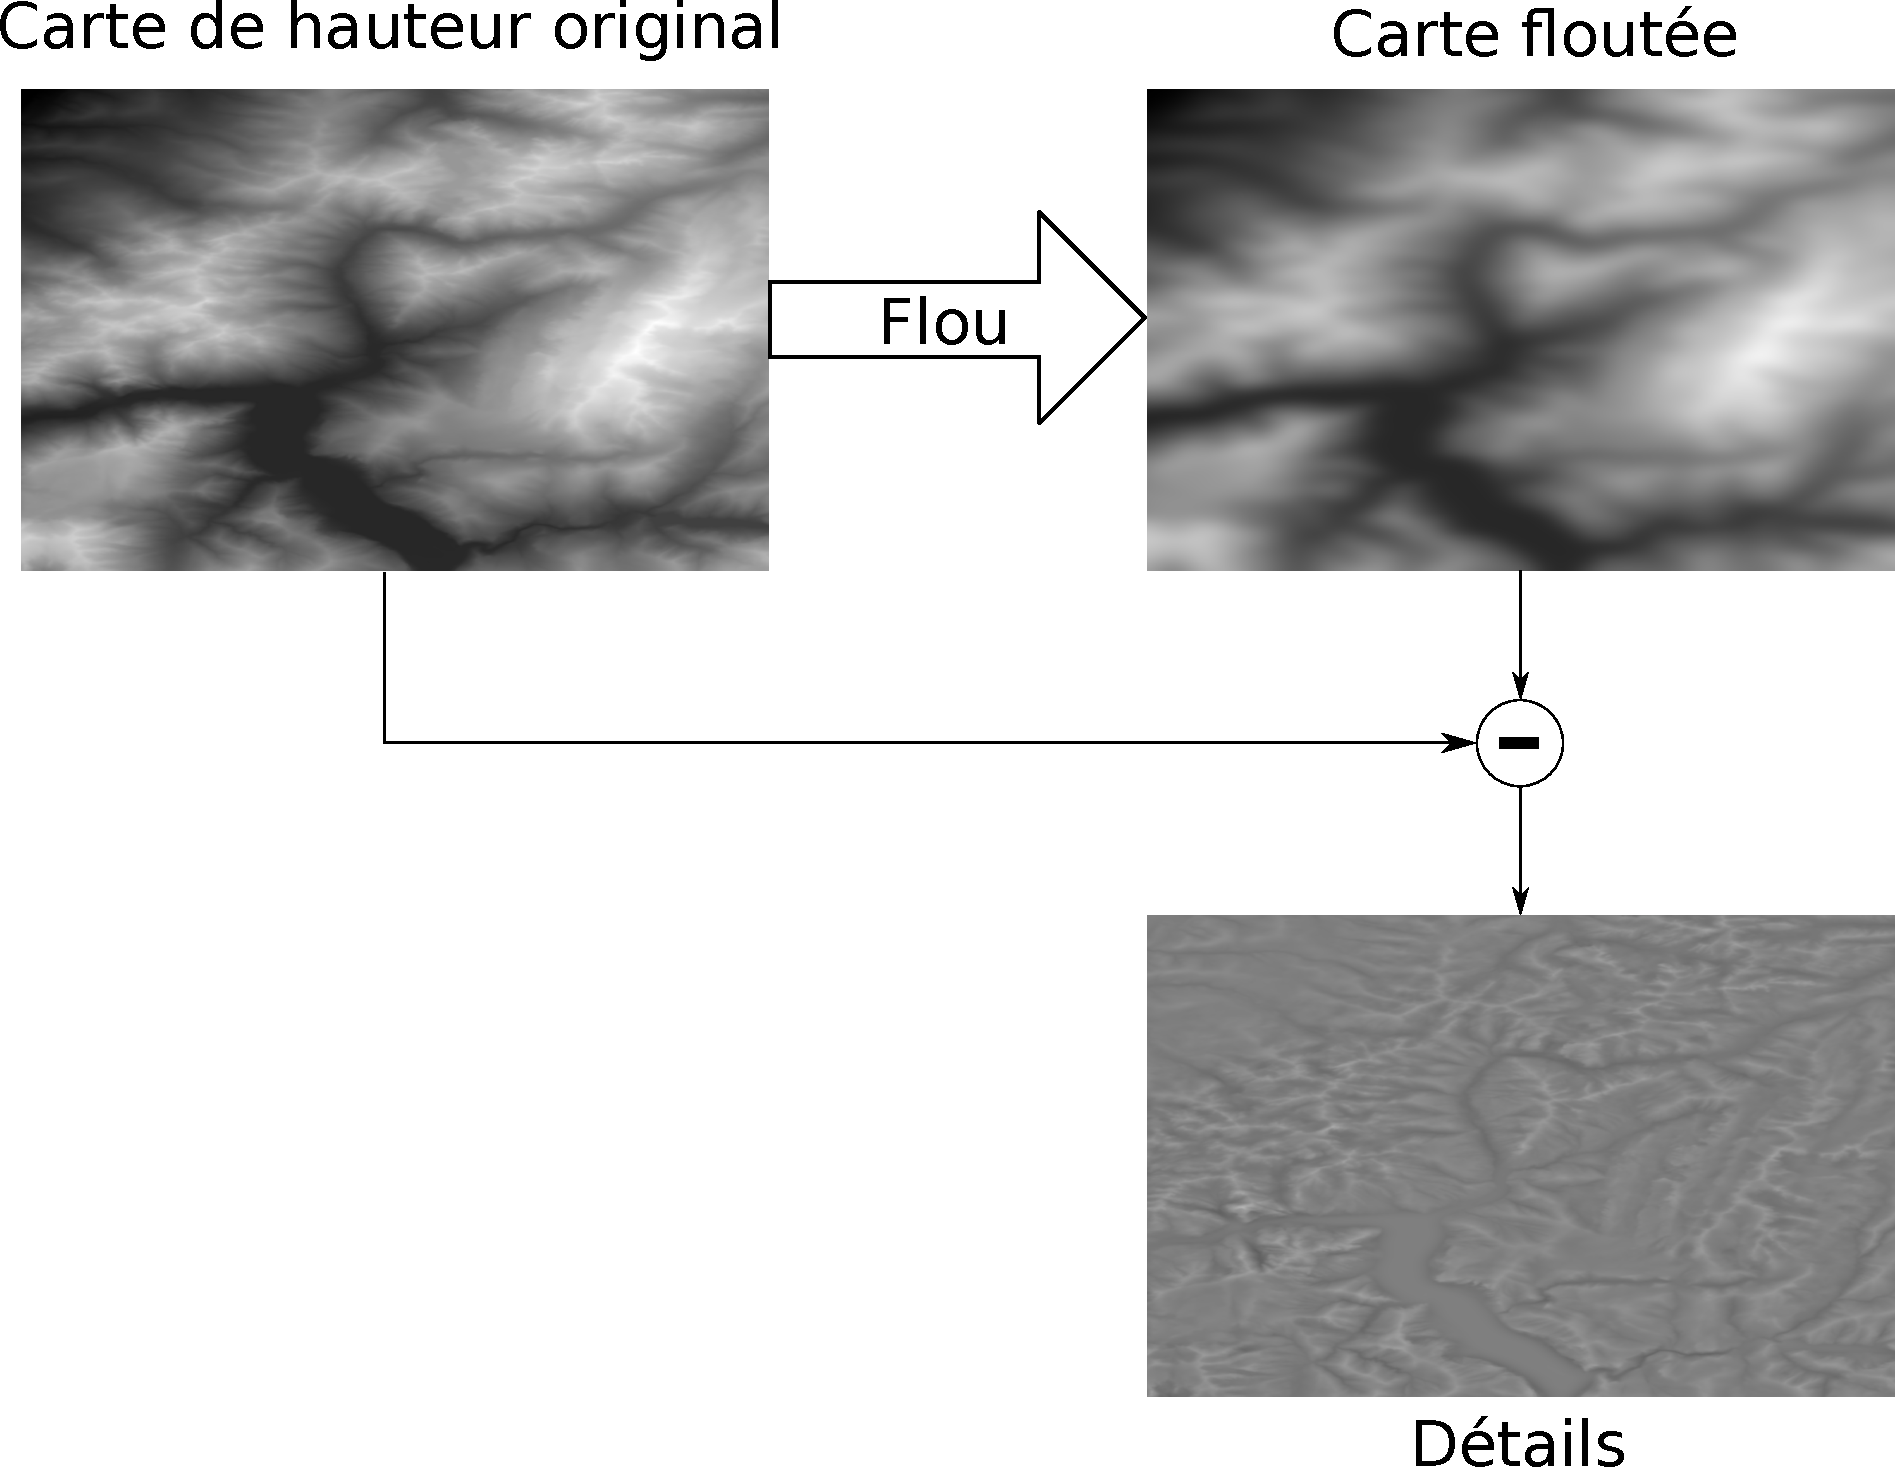
\includegraphics[width=1.0\linewidth]{Solution/pyramide_Laplace_image.pdf}
 \caption{Deux dimensions}
 \end{subfigure}
 \caption{\label{fig:pyramide} Pyramide Laplacienne sur une carte de hauteur}
\end{figure*}
La solution est donc d'utiliser un système multi-échelle pour permettre aux détails de ressortir. Notre solution consiste à utiliser une pyramide Laplacienne \cite{adelson1984pyramid} pour produire deux échelles. Le principe est de produire à l'aide d'un flou gaussien une version floutée de la carte de hauteur et ensuite de faire la différence entre la carte originale et la version floutée (Fig \ref{fig:pyramide})
Le flou gaussien s'obtient en convoluant chaque point de la carte de hauteurs par une gaussienne en deux dimensions : 
\begin{equation}
G(x,y,\sigma) = \frac{1}{2\pi\sigma^2}e^{-\frac{x^2+y^2}{2\sigma^2}},
\end{equation}
avec $x$ et $y$ la distance par rapport à l'origine et $\sigma$ l’écart type de la gaussienne.


\begin{figure}
\centering
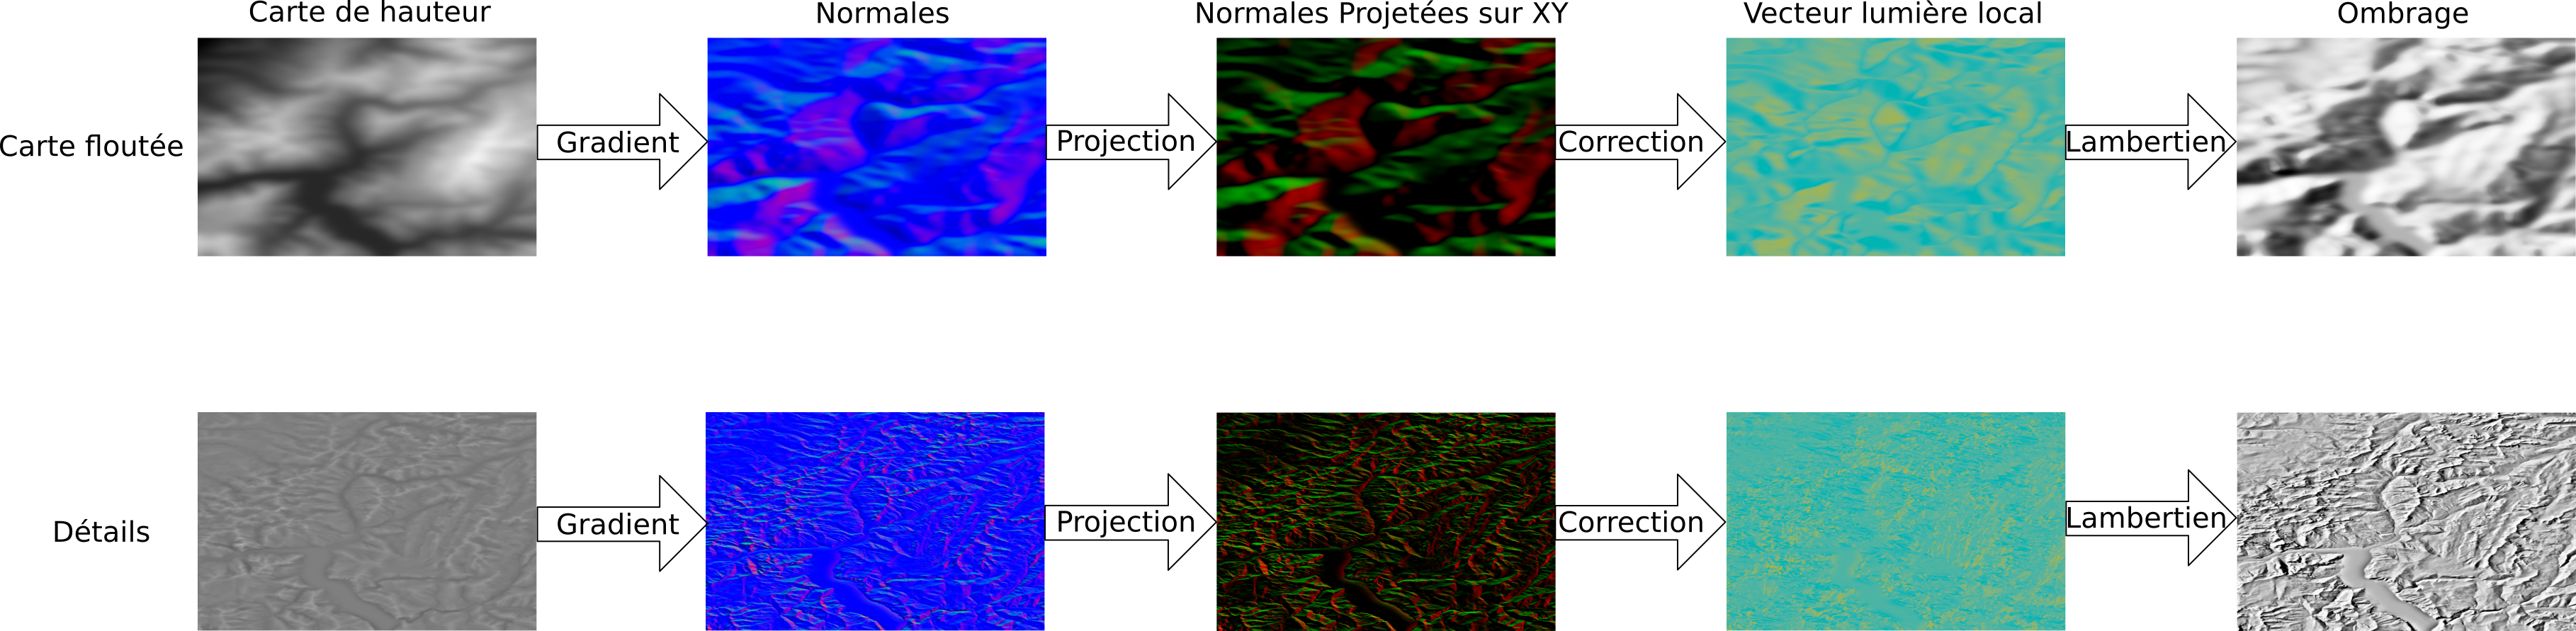
\includegraphics[width=1.0\linewidth]{Solution/pyramide_Laplace_image_extended.png}

\caption{\label{fig:pyramide_extended}Les différentes étapes de notre méthode pour générer l'ombrage sur deux échelles}
\end{figure}




Une fois ces deux échelles obtenues, nous extrayons les normales puis nous calculons l'orientation de la lumière localement de manière indépendante afin de calculer un ombrage. (Fig. \ref{fig:pyramide_extended}).  


\section{Fusion des ombrages}
Les deux ombrages de chaque échelles obtenues, il faut maintenant les fusionner afin d'obtenir un unique ombrage pour le rendu final. Cependant cette fusion n'est pas triviale. En effet, la manière de fusionner va influencer la quantité de détails perçus et le style final du rendu. Ainsi, une simple interpolation linéaire ne permet pas de répondre correctement à la problématique de percevoir la maximum de détails tout en gardant le contraste et la nervosité du style Novat. 

Parmi les fonctions de fusion qui existent, celles de type \textit{Overlay} répondent à notre problématique. L'idée principale de ces fonctions est de partir d'un niveau de gris compris entre 0 et 1 (dans notre cas, l'ombrage de la partie détaillée $d$) et de lui appliquer un $2^e$ niveau de gris (dans notre cas, l'ombrage de la partie floutée $f$) pour faire faire varier le $1^{er}$ niveau de gris. Ça a pour avantage d'avoir un niveau de gris principal et un secondaire. Nous utilisons celle utilisée dans le rendu d'aquarelle de Bousseau et al. \cite{bousseau2006interactive} (équation  \ref{equationAquarelle} et Fig. \ref{fig:watercolorcurve}) qui a pour avantage de n'enlever aucune aspérité tout en augmentant le contraste de l'ombrage (cf Fig. \ref{fig:comparaisonFusion}).
\begin{equation}
\label{equationAquarelle}
        A(d,f) = d - (d -d^2)( 1-2f) 
\end{equation}
\begin{figure}[h!]
\centering
        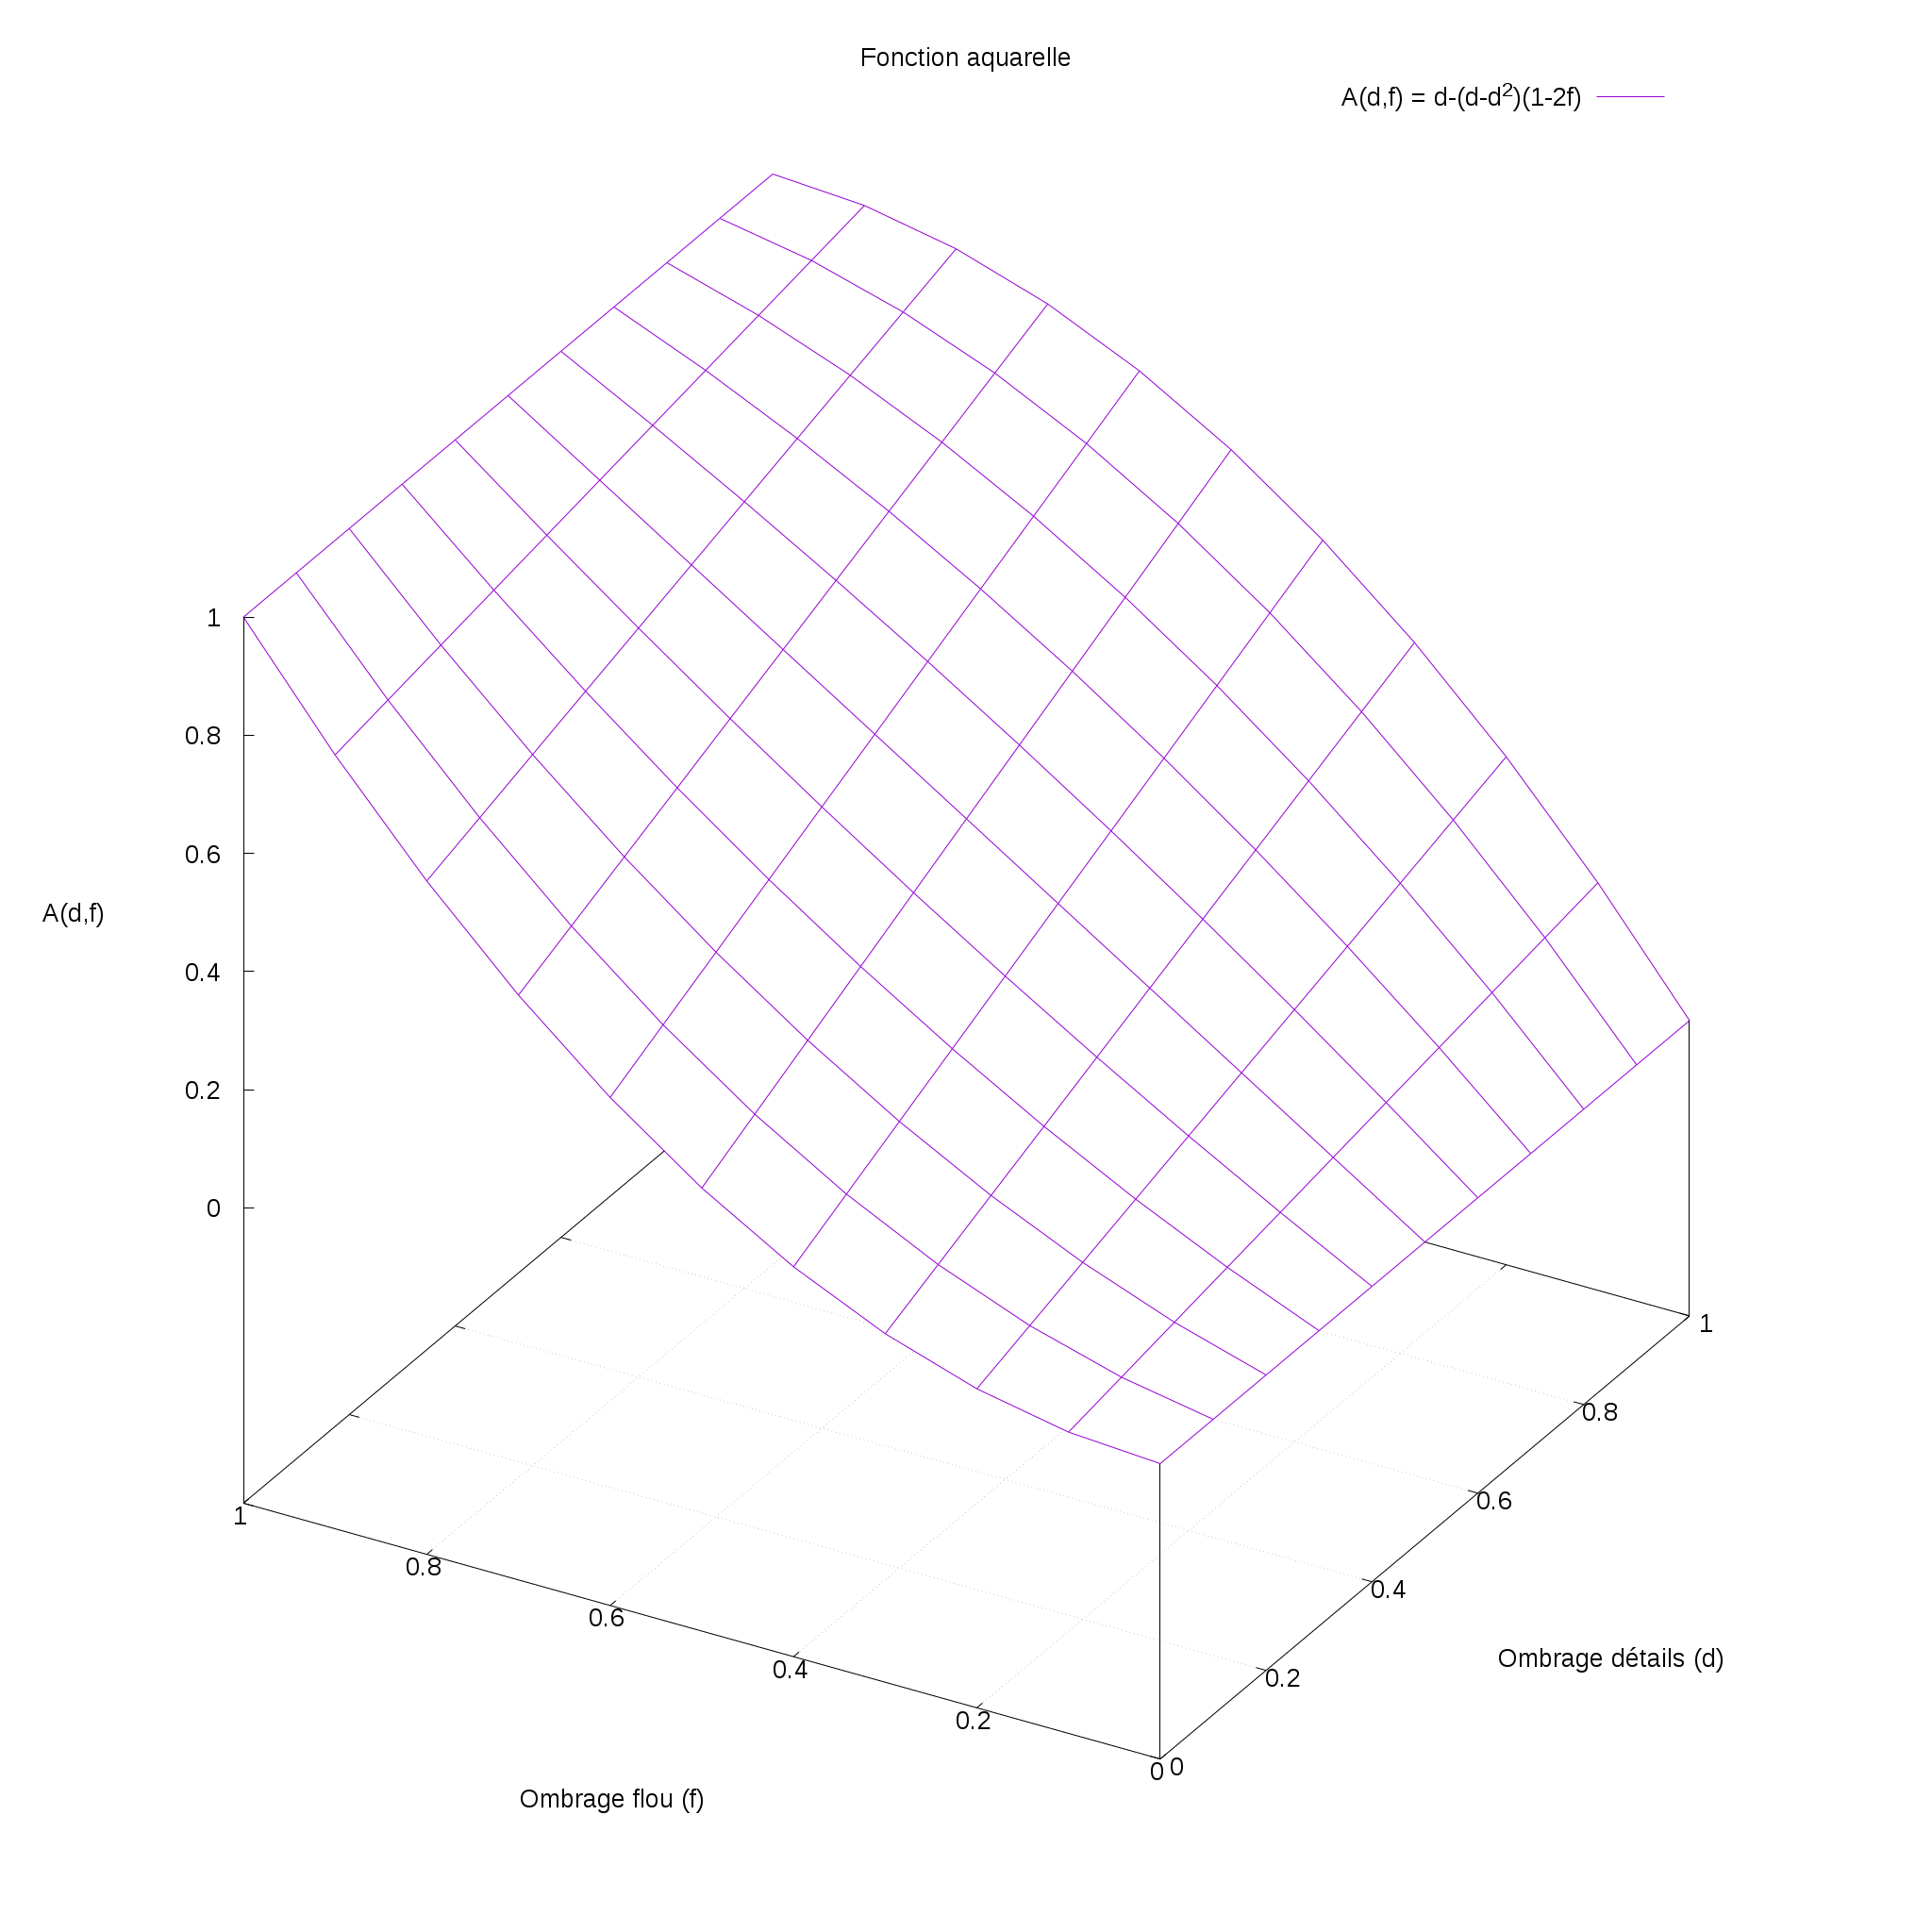
\includegraphics[width=0.5\linewidth]{Solution/watercolor_curve}
        \caption{\label{fig:watercolorcurve} Courbe de la fonction $A(d,f)$}

\end{figure}

\begin{figure*}[!h]
\centering
 \begin{subfigure}[t]{0.32\linewidth}
 \centering
 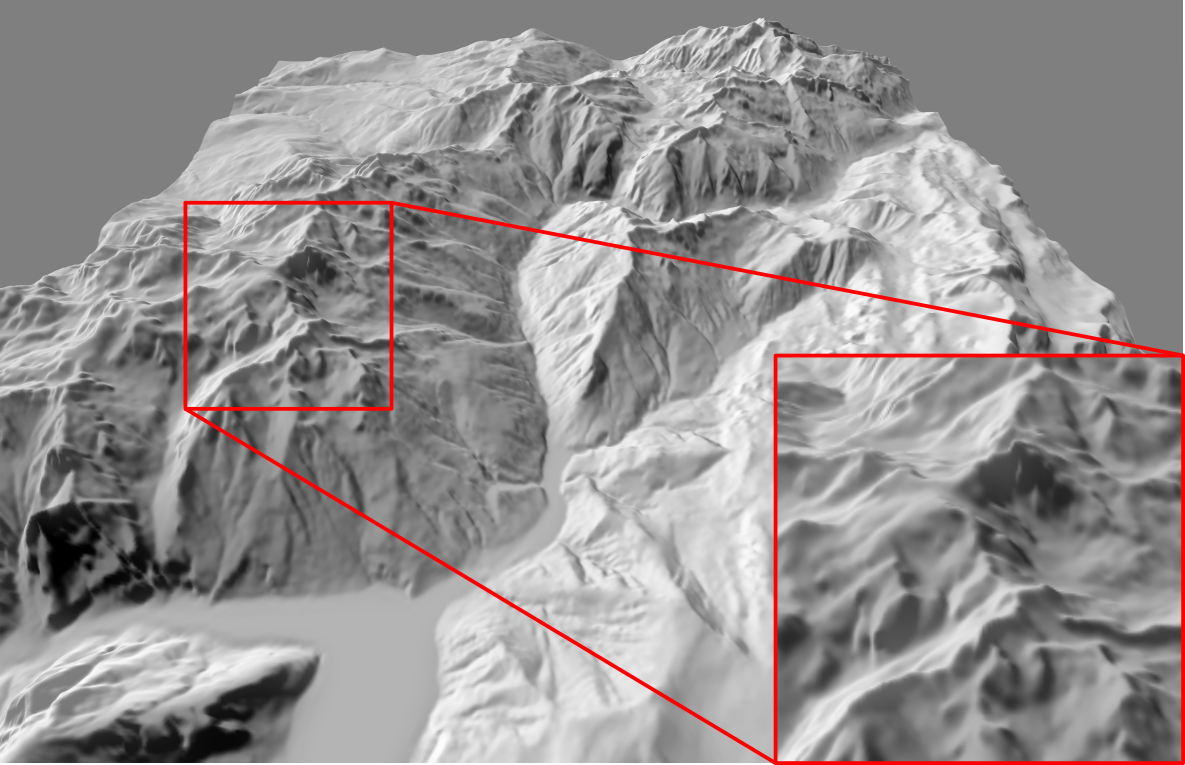
\includegraphics[width=1.0\linewidth]{Solution/ShadeLineaire.png}
 \caption{Interpolation linéaire }
 \end{subfigure}
 \begin{subfigure}[t]{0.32\linewidth}
 \centering
 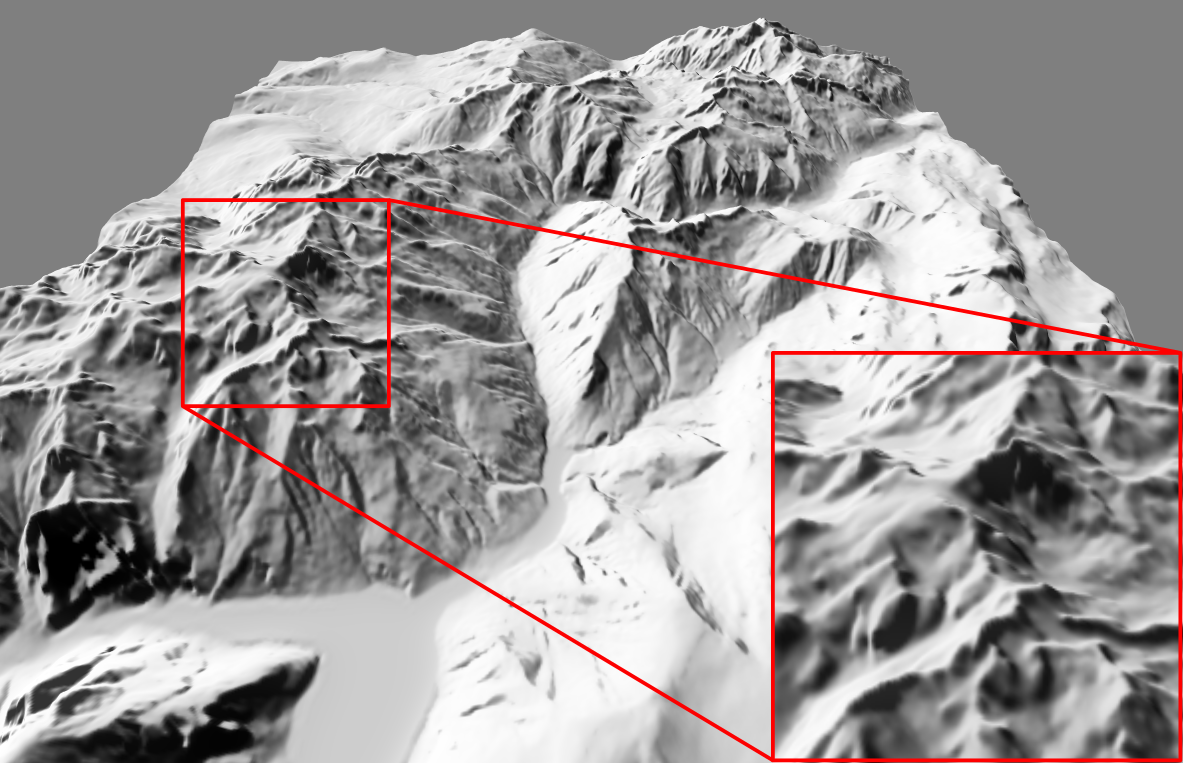
\includegraphics[width=1.0\linewidth]{Solution/ShadeOverlay.png}
  \caption{Overlay de Gimp et photoshop }
 \end{subfigure}
  \begin{subfigure}[t]{0.32\linewidth}
 \centering
 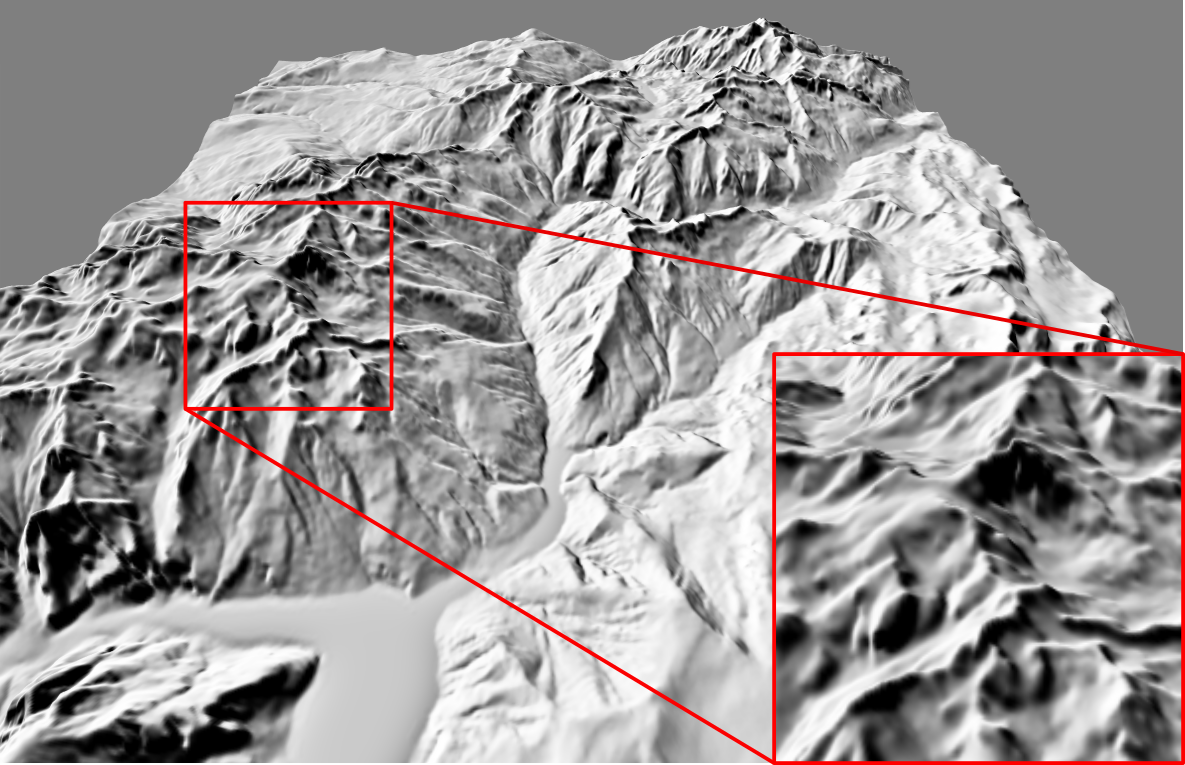
\includegraphics[width=1.0\linewidth]{Solution/ShadeWatercolor.png}
  \caption{Fonction aquarelle de Bousseau et al. \cite{bousseau2006interactive}}
 \end{subfigure}
 \caption{\label{fig:comparaisonFusion} Comparaison entre différente type de fusion.($\alpha =  270\degres$ (Est), $\gamma = 45\degres$ , $\sigma = 30$) Nous observons que les deux fonction \textit{overlay} font plus ressortir l'ombrage, cependant la méthode "aquarelle" évite de perdre certaines aspérités lorsqu'elles sont dans une partie très éclairée ou très sombre.}
\end{figure*}


\section{Les ombres portées}
\subsection{Calcul des ombres portées}
Les ombres portées ne sont pas calculées de la même manière que l'ombrage. Pour ces ombres-là, l'information nécessaire est : quelle est la forme de l’objet qui bloque la lumière. Pour ce faire il existe différentes techniques (shadow maps, shadow volume, etc..), nous renvoyons le lecteur à l'état de l'art \cite{woo1990survey} pour plus d'information. Celle qui nous intéresse est une technique dite de \textit{Ray Marching}. Elle a pour avantage d'être facilement applicable sur une carte de hauteur et permet d'avoir un vecteur de lumière différent par point. 
Le principe est assez simple : en chaque point nous laçons un rayon dans la direction de la lumière et nous vérifions s'il intercepte un objet ou non. Dans notre cas, comme nous partons d'une carte de hauteur, nous avançons pas par pas et nous vérifions si nous sommes en dessous ou non de la hauteur du point courant. Cela permet d'obtenir une carte  où $1$ indique que la lumière passe et $0$ l'inverse (Fig. \ref{fig:raymarching}). 


\begin{figure}
\centering
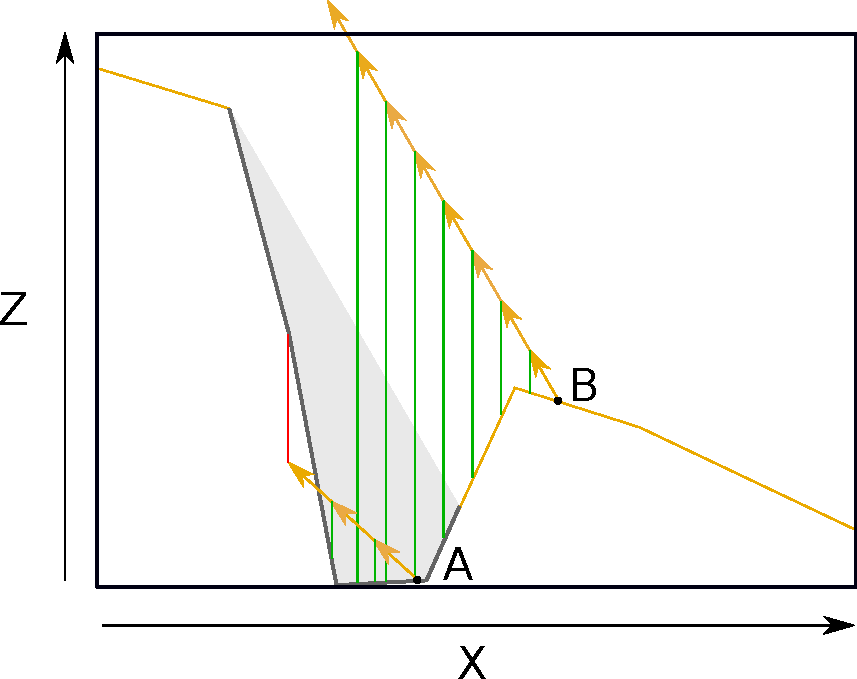
\includegraphics[width=0.5\linewidth]{Solution/raymarching.pdf}
\caption{\label{fig:raymarching} Raymarching sur deux pixel A et B avec en jaune les vecteurs lumières et en vert et rouge la distance par rapport au terrain après chaque pas. A est dans l'ombre, B est dans la lumière}
\end{figure}
\subsection{Abstraction des ombres portées }

Cependant la forme des ombres obtenues n'est pas vraiment conforme au style Novat. Dans les panoramas les ombres portées sont très anguleuses et très marquées or les nôtres se basent sur la forme du terrain qui est plus continue. Parmi les filtres possibles pour transformer la carte des ombres portées, il y a la morphologique mathématique qui est utilisée pour abstraire les formes (utilisée par exemple par Bousseau et al. dans leur rendu aquarelle \cite{bousseau2006interactive}). Cela consiste à traiter un ensemble $A$ à l'aide d'un autre ensemble $B$ appelé élément structurant qui sert de sonde. Pour chaque position de l’élément structurant, nous vérifions s'il est inclus ou non dans l'ensemble initial. À partir de cette information, et d'un opérateur, nous construisons un ensemble de sortie. De notre coté , nous utilisons l’opérateur de fermeture de $A$ par $B$ qui est la succession de l’opérateur de dilatation de $A$ par $B$ suivit de l’opérateur d’érosion du résultat par $B$ :
\begin{equation} 
A \bullet B  = (A \oplus B) \ominus B
\end{equation}
Avec l’opérateur d’érosion : 
\begin{equation} 
A \ominus B  = \{ x \mid \forall a \in A, B_a \cap A = \emptyset   \}
\end{equation}
Et l’opérateur de dilatation : 
\begin{equation} 
A \oplus B  = \{x \mid \forall a \in A, B_a \cap A \neq \emptyset  \}
\end{equation}
Avec x les pixels de l'image et $B_a$ qui correspond à $B$ centré en $a$. 



Dans notre solution $A$ représente l'ensemble des pixels dans l'ombre $(=0)$ et nous utilisons un carré de $5x5$ pixels comme élément structurant (Fig \ref{fig:pyramide_morpho} et \ref{fig:comparaisonMorpho}).
\begin{figure}[h!]
\centering
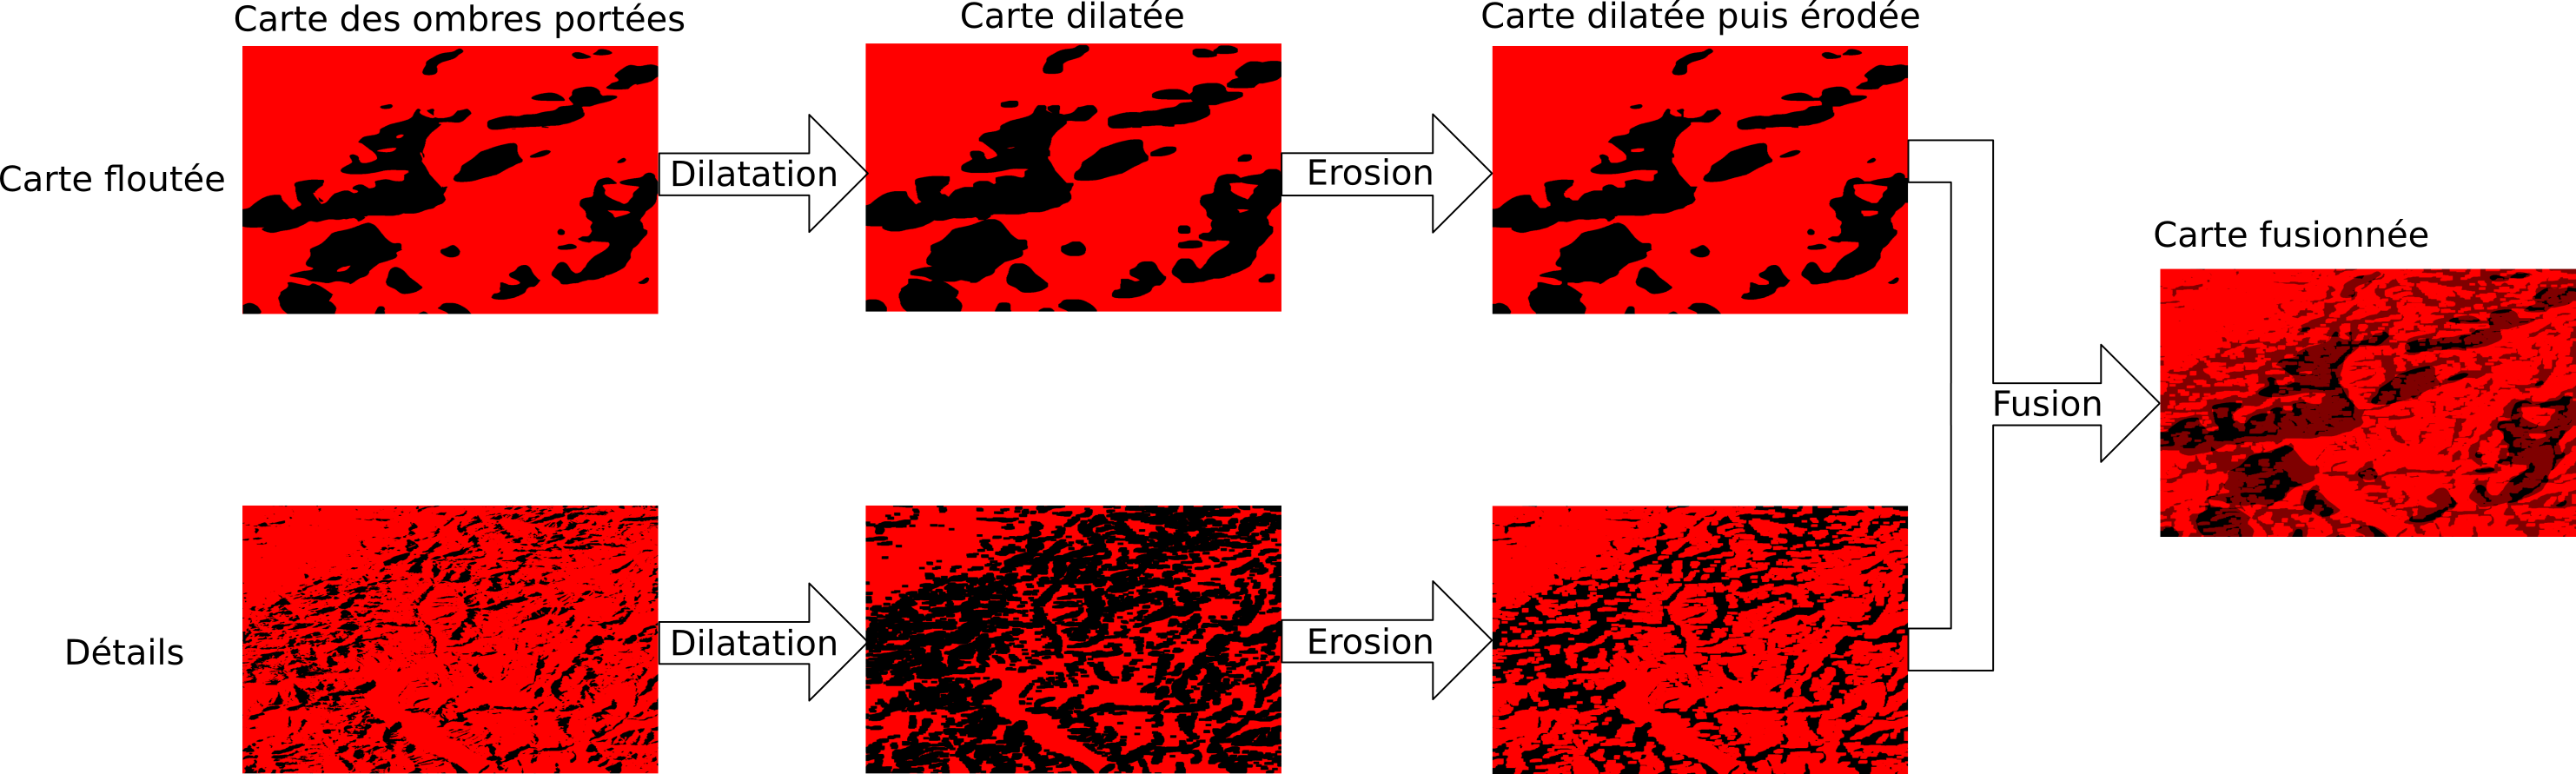
\includegraphics[width=1.0\linewidth]{Solution/pyramide_Laplace_image_morpho.png}

\caption{\label{fig:pyramide_morpho}L'ouverture puis la fusion des ombres portées}
\end{figure}


\begin{figure*}[h!]
\centering
 \begin{subfigure}[t]{0.47\textwidth}
 \centering
 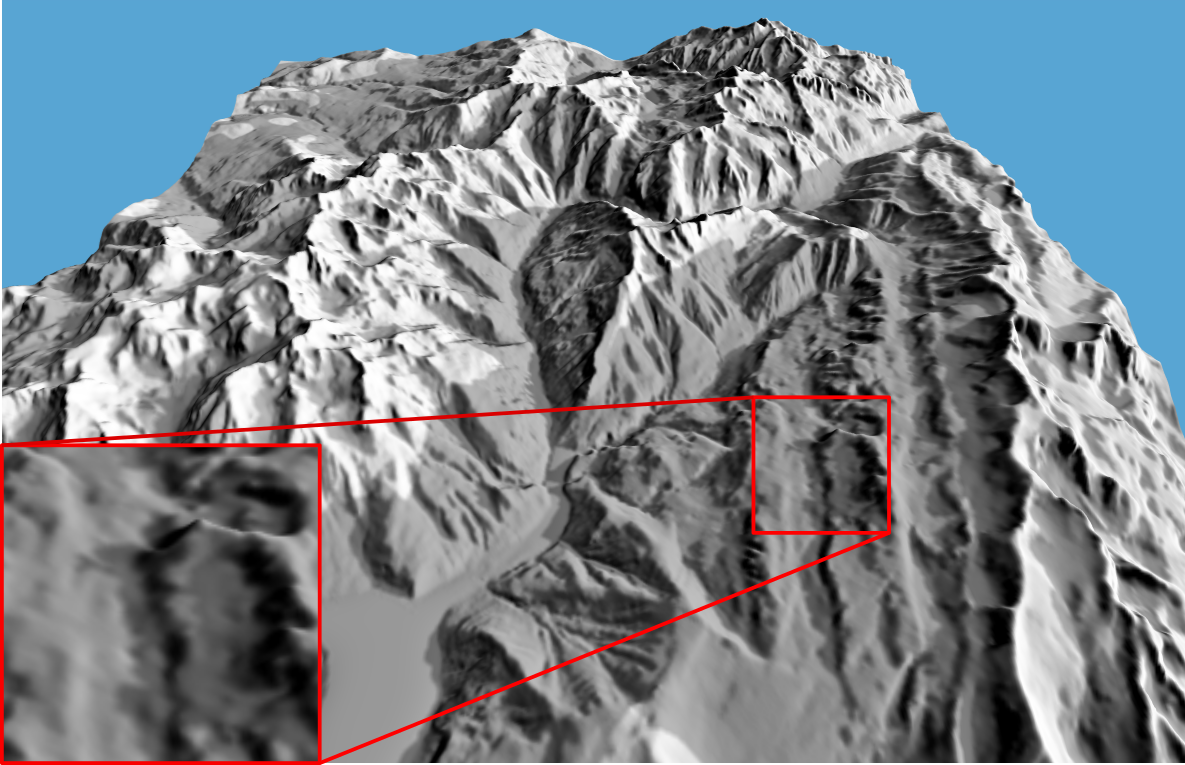
\includegraphics[width=1.0\linewidth]{Solution/sansMorpho.png}
 \caption{Sans abstraction des formes}
 \end{subfigure}
 \begin{subfigure}[t]{0.47\textwidth}
 \centering
 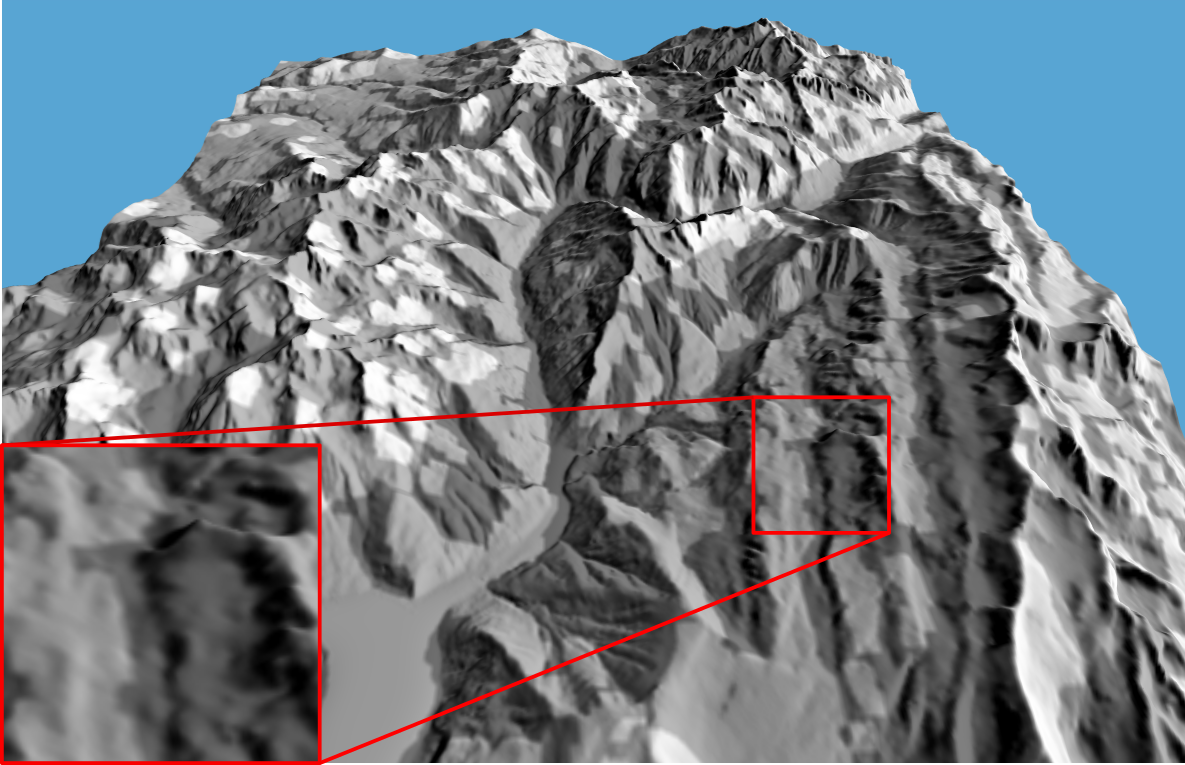
\includegraphics[width=1.0\linewidth]{Solution/avecMorpho.png}
 \caption{Avec abstraction des formes}
 \end{subfigure}
 \caption{\label{fig:comparaisonMorpho} Comparaison avec et sans abstraction des formes avec la morphologie mathématique ($\alpha =  270\degres$ (Est), $\gamma = 10\degres$ , $\sigma = 30$).}
\end{figure*}
\clearpage
\subsection{Multi Échelles et fusion}

Nous utilisons la même méthode pour les ombres portées qu'avec l'ombrage, c'est-à-dire que nous utilisons les deux mêmes échelles pour générer les ombres portées de manière indépendante pour les fusionner ensuite. Cependant la technique de fusion n'est pas la même. En effet, comme les cartes des ombres portées ne sont composées que de 0 et de 1, une simple interpolation linéaire suffit à faire une fusion acceptable. 


Enfin nous fusionnons les ombres portées avec l'ombrage avec l’équation \ref{equationFusionOMOP} qui permet d'ajouter de manière discrète les ombres portées sans masquer la variation de l'ombrage (voir Figure \ref{fig:shadow_shade}). 
\begin{equation}
\label{equationFusionOMOP}
O = OM . \frac{OP+1}{2}
\end{equation} 
Avec $OP$ la valeur des ombres portées au pixel courant, $OM$ la valeur de l'ombrage sur ce même pixel et $O$ l’ombrage final.

\begin{figure}[h!]
\centering
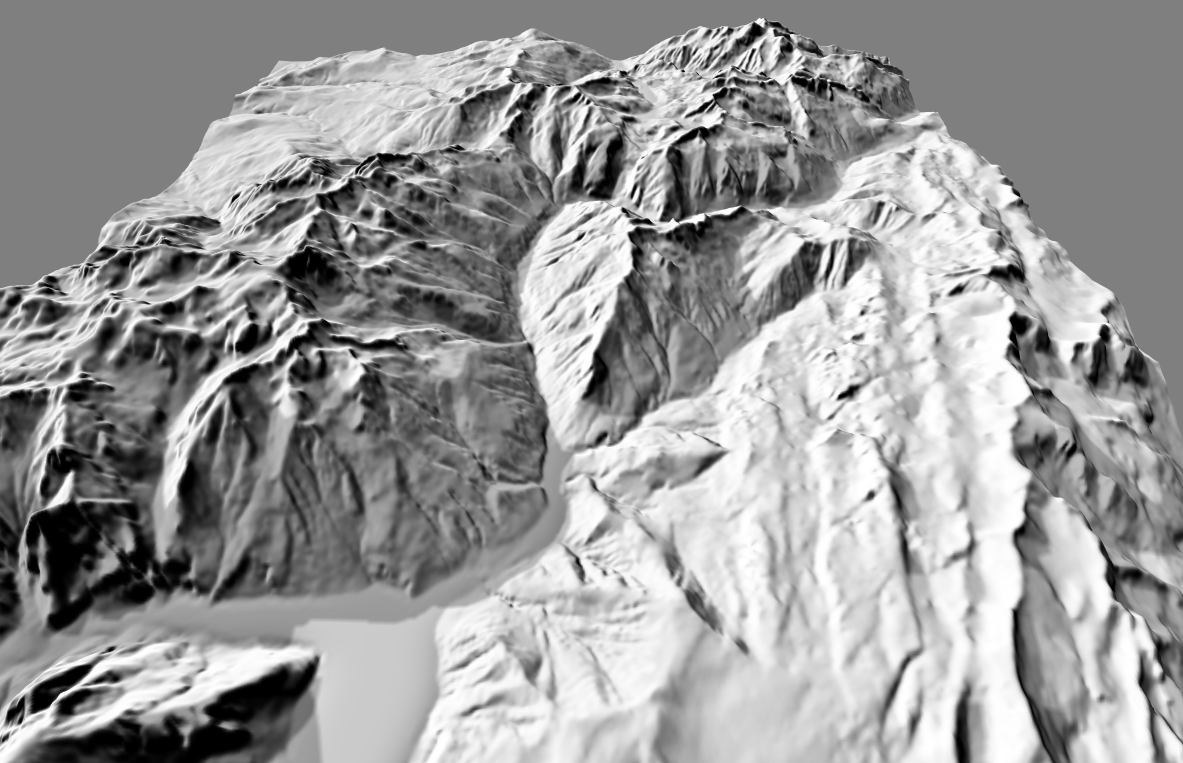
\includegraphics[width=1.0\linewidth]{Solution/shadow_shade.png}
\caption{\label{fig:shadow_shade}Fusion de l'ombrage avec les ombres portées. ($\alpha =  45\degres$ (Nord-Ouest), $\gamma = 20\degres$ , $\sigma = 30$)}
\end{figure}




